\documentclass[border=1in]{standalone}
\usepackage{tikz}
\usetikzlibrary{arrows}

% ensures a white background in the converted image
\pagecolor{white}

\begin{document}
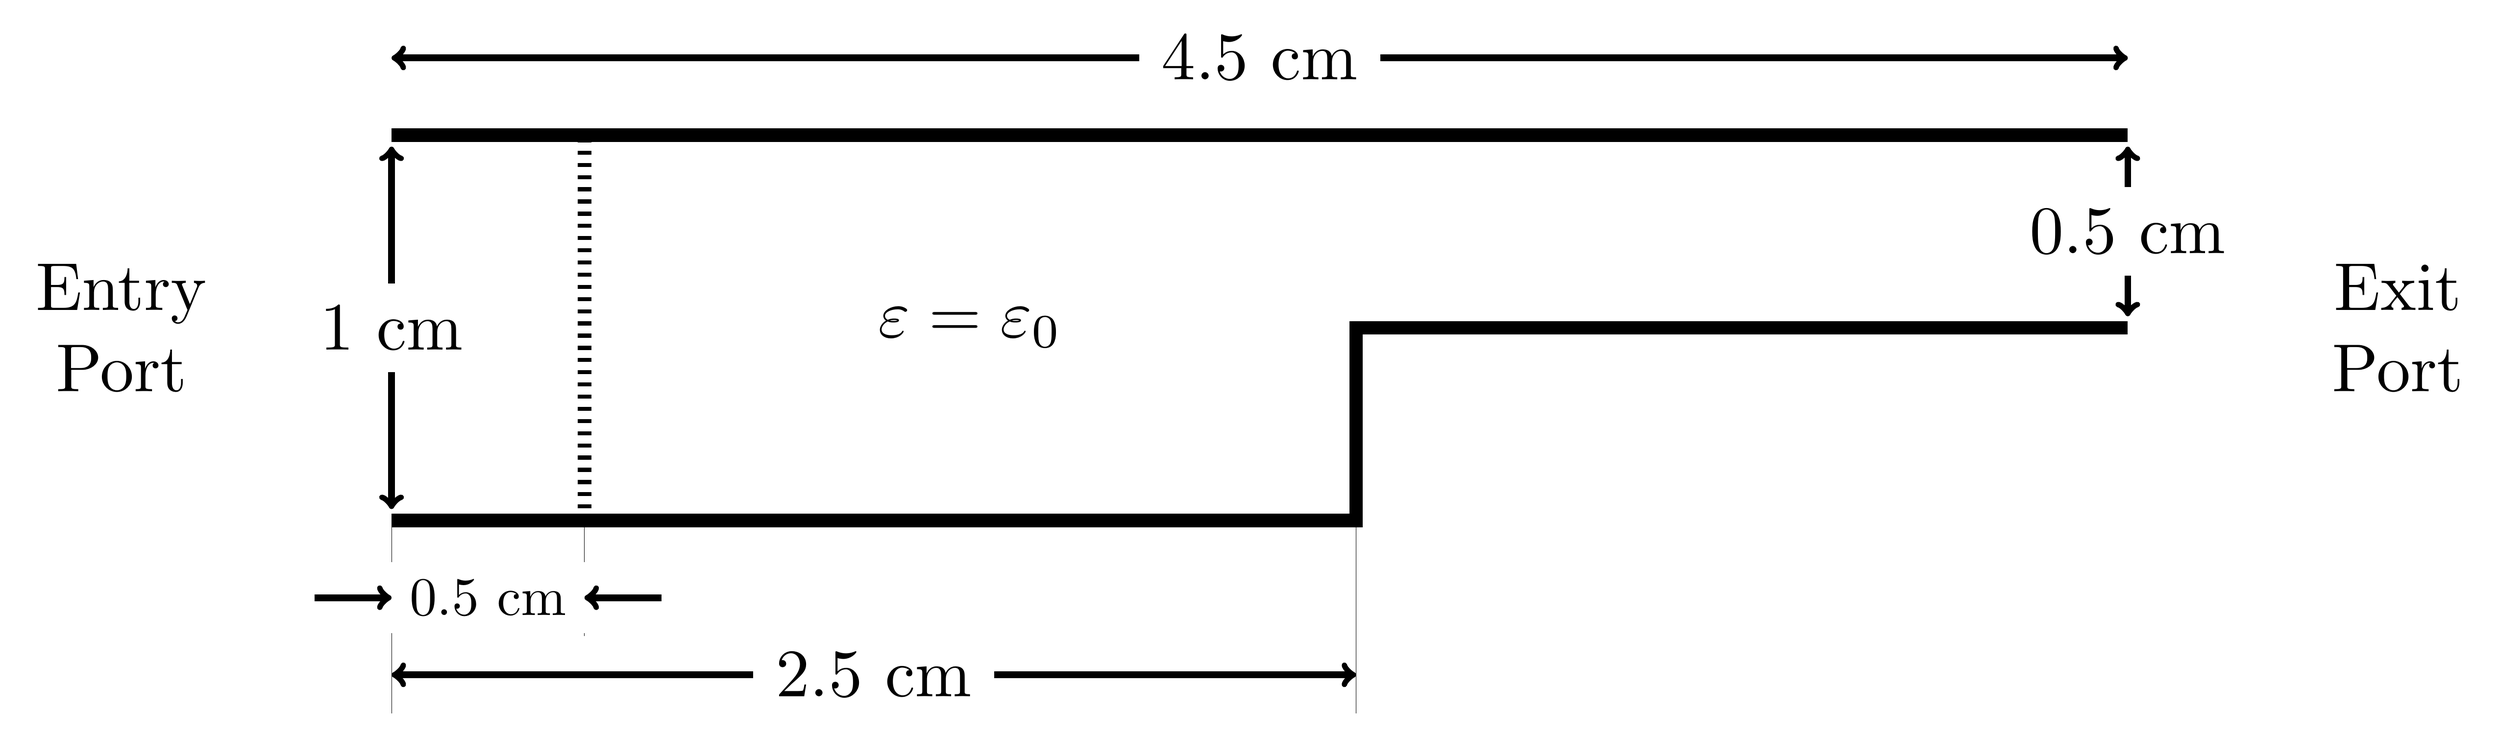
\begin{tikzpicture}
  % Draw lines
  \draw [line width=10pt] (0, 10) -- (45, 10);
  \draw [line width=10pt] (0, 0) -- (25, 0) -- (25, 5) -- (45, 5);
  \draw [line width=10pt, loosely dashed] (5, 0) -- (5, 10);
  % Draw width arrows (with lines for entry port side)
  \draw[arrows=<->, line width=5pt] (0, 0.3) -- (0, 9.7);
  %\draw (-3, 0) -- (0, 0);
  %\draw (-3, 10) -- (0, 10);
  \draw[arrows=<->, line width=5pt] (45, 5.3) -- (45, 9.7);
  % Add widths
  \node [fill=white, scale=5] at (0, 5) {1 cm};
  \node [fill=white, scale=5] at (45, 7.5) {0.5 cm};
  % Draw length arrows (with lines for bottom side)
  \draw[arrows=<->, line width=5pt] (0, -4) -- (25, -4);
  \draw (0, 0) -- (0, -5);
  \draw (25, 0) -- (25, -5);
  \draw[arrows=->, line width=5pt] (-2, -2) -- (0, -2);
  \draw[arrows=<-, line width=5pt] (5, -2) -- (7, -2);
  \draw (5, 0) -- (5, -3);
  \draw[arrows=<->, line width=5pt] (0, 12) -- (45, 12);
  % Add legnths
  \node[fill=white, scale=5] at (12.5, -4) {2.5 cm};
  \node[fill=white, scale=4] at (2.5, -2) {0.5 cm};
  \node[fill=white, scale=5] at (22.5, 12) {4.5 cm};
  % Add vacuum label
  \node[fill=white, scale=5] at (15, 5) {$\varepsilon = \varepsilon_0$};
  % Add port labels
  \node[fill=white, scale=5, align=center] at (-7, 5) {Entry\\Port};
  \node[fill=white, scale=5, align=center] at (52, 5) {Exit\\Port};
\end{tikzpicture}
\end{document}
